\documentclass[thesis.tex]{subfiles}

 
\begin{document}
\chapter{Experimental Apparatus}
\label{ch2}

\section{The Large Hadron Collider}
The Large Hadron Collider (LHC)~\cite{LHCTDR}, located at CERN on the France-Switzerland border, is currently the world's largest particle accelerator and collider. 
It is installed in a 27 km long near-circular tunnel that was constructed in the 1980s to host the Large Electron-Positron (LEP) machine. 
The LHC uses twin-bore magnets to allow two proton beams to travel in opposite directions. 
The main superconducting magnets of the LHC operate at a temperature below 2K, which is maintained by a superfluid helium cryogenic system, and generates a peak dipole field of 8.33 T. 
The LHC is designed to provides a peak luminosity of $L = 10^{34}cm^{2}s^{-1}$ and a maximum center of mass energy of $\sqrt{s} = $14 TeV for proton-proton collisions. 

The protons injected to the LHC are boosted by a chain of accelerators, each of which increases the energy of the protons to a certain scale and the beams can also be delivered to other experiments at low energy. 
The configuration of the CERN accelerator complex is shown in Fig. \ref{fig:LHC}. 
At the first stage, the protons extracted from a bottle of hydrogen gas are fed into the LINAC 2, a linear accelerator, and are boosted to the energy of 50 MeV.  
The beams are then injected to the Proton Synchrotron Booster, followed by the Proton Synchrotron (PS), which brings the protons to 25 GeV. 
The Super Proton Synchrotron (SPS) then accelerates the proton beams to 450 GeV and injects them into the LHC. 
The LHC is the last element in the accelerator complex, where protons are stored and accelerated to the designed energy.

\begin{figure*}[hbt]
	\centering
	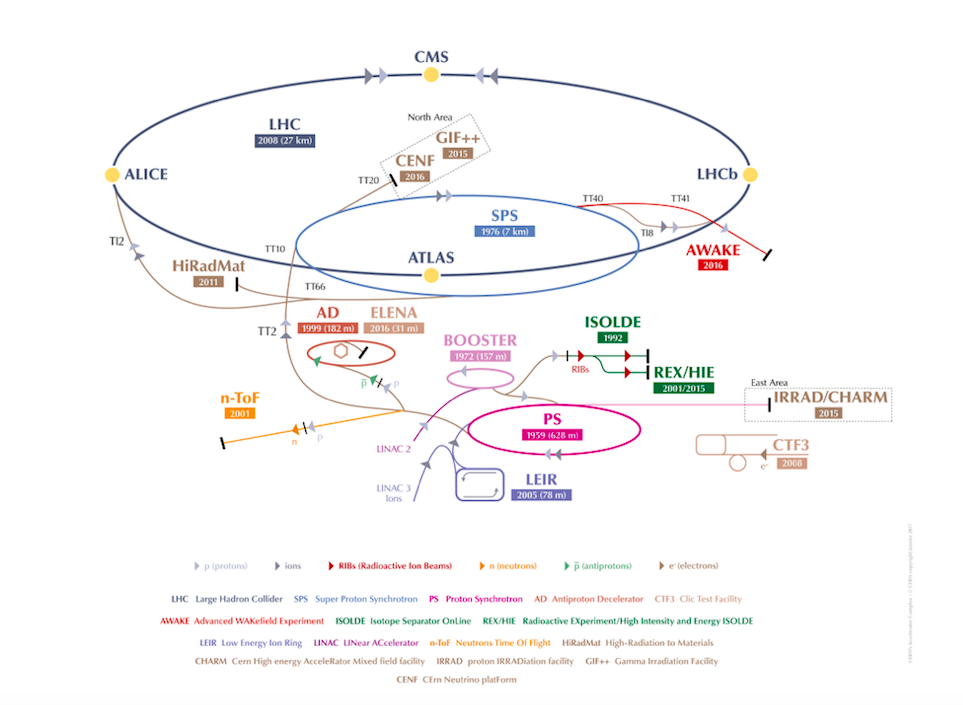
\includegraphics[width=0.8\textwidth]{plot/LHCcomplex.png}
	\caption{Scheme of the CERN Accelerator Complex.}
	\label{fig:LHC}
\end{figure*}


The two high-energy proton beams circulate in the LHC at close to the speed of light and collide with each other at four interaction points (IP), corresponding to the location of the four detectors: CMS, ATLAS, ALICE and LHCb. 
The CMS and ATLAS are general-purpose detectors, which investigate a wide range of physics from the precise measurements of the SM to searches for new physics. 
The ALICE is a heavy-ion detector, focusing on the study of strong interactions. 
The LHCb experiment specializes in b quark physics, and it is a single arm detector which mainly collects forward particles. 
In addition, there are three smaller experiments on the LHC: TOTEM (Total, elastic and diffractive cross-section measurement), LHCf ((Large Hadron Collider forward) and MoEdal (Monopole and Exotics Detector). 
This thesis will focus on the results of the CMS experiments. 

\section{The CMS Detector}

The Compact Muon Solenoid (CMS) experiment is a hermetic, general-purpose detector located at the collision point 5 of the LHC.  It is 21.6 m long, 15 m high, 15 m in diameter, and weighs about 12,500 tons. The physics goal is to investigate a wide range of phenomena including the study of the Higgs mechanism and searches for unknown particles beyond the SM. The cross-section of the interesting physics process is typically 5-10 order of magnitude smaller than the total cross-section, making it crucial to measure the momentum and time of the particles with high resolution. To meet the physics goals, the detector is designed to fulfill the following requirements:   
\begin{itemize}
\item good muon identification and high momentum resolution;
\item good electromagnetic energy resolution;
\item efficient tracking and accurate momentum measurements for charged particles;
\item good missing transverse momentum resolution, requiring hadron calorimeters with a large hermetic geometric coverage. 
\end{itemize}

To satisfy these requirements, a 13 m long, 6 m inner diameter superconducting solenoid is built to generate a magnetic field of 4 T, providing large bending power to precisely measure the momentum of charged particles. The coil is cooled by liquid helium to operate at a temperature of 4.5 K. The flux is returned through a steel yoke consisting of five barrel wheels and four end-cap disks at each end. 

Figure \ref{fig:cmslayout} shows an overview of the layout of the CMS detector. Close to the interaction point is a high granular three-layer silicon pixel detector which improves the track and vertex reconstruction, followed by a silicon strip tracker. Surrounding it is a lead-tungstate crystal electromagnetic calorimeter (ECAL) and a brass/scintillator sampling hadron calorimeter (HCAL). The tracker and calorimeter are compact enough to fit into the bore of the magnet coil. Outside the solenoid are the muon stations, embedded in the return yoke. 

\begin{figure*}[hbt]
	\centering
	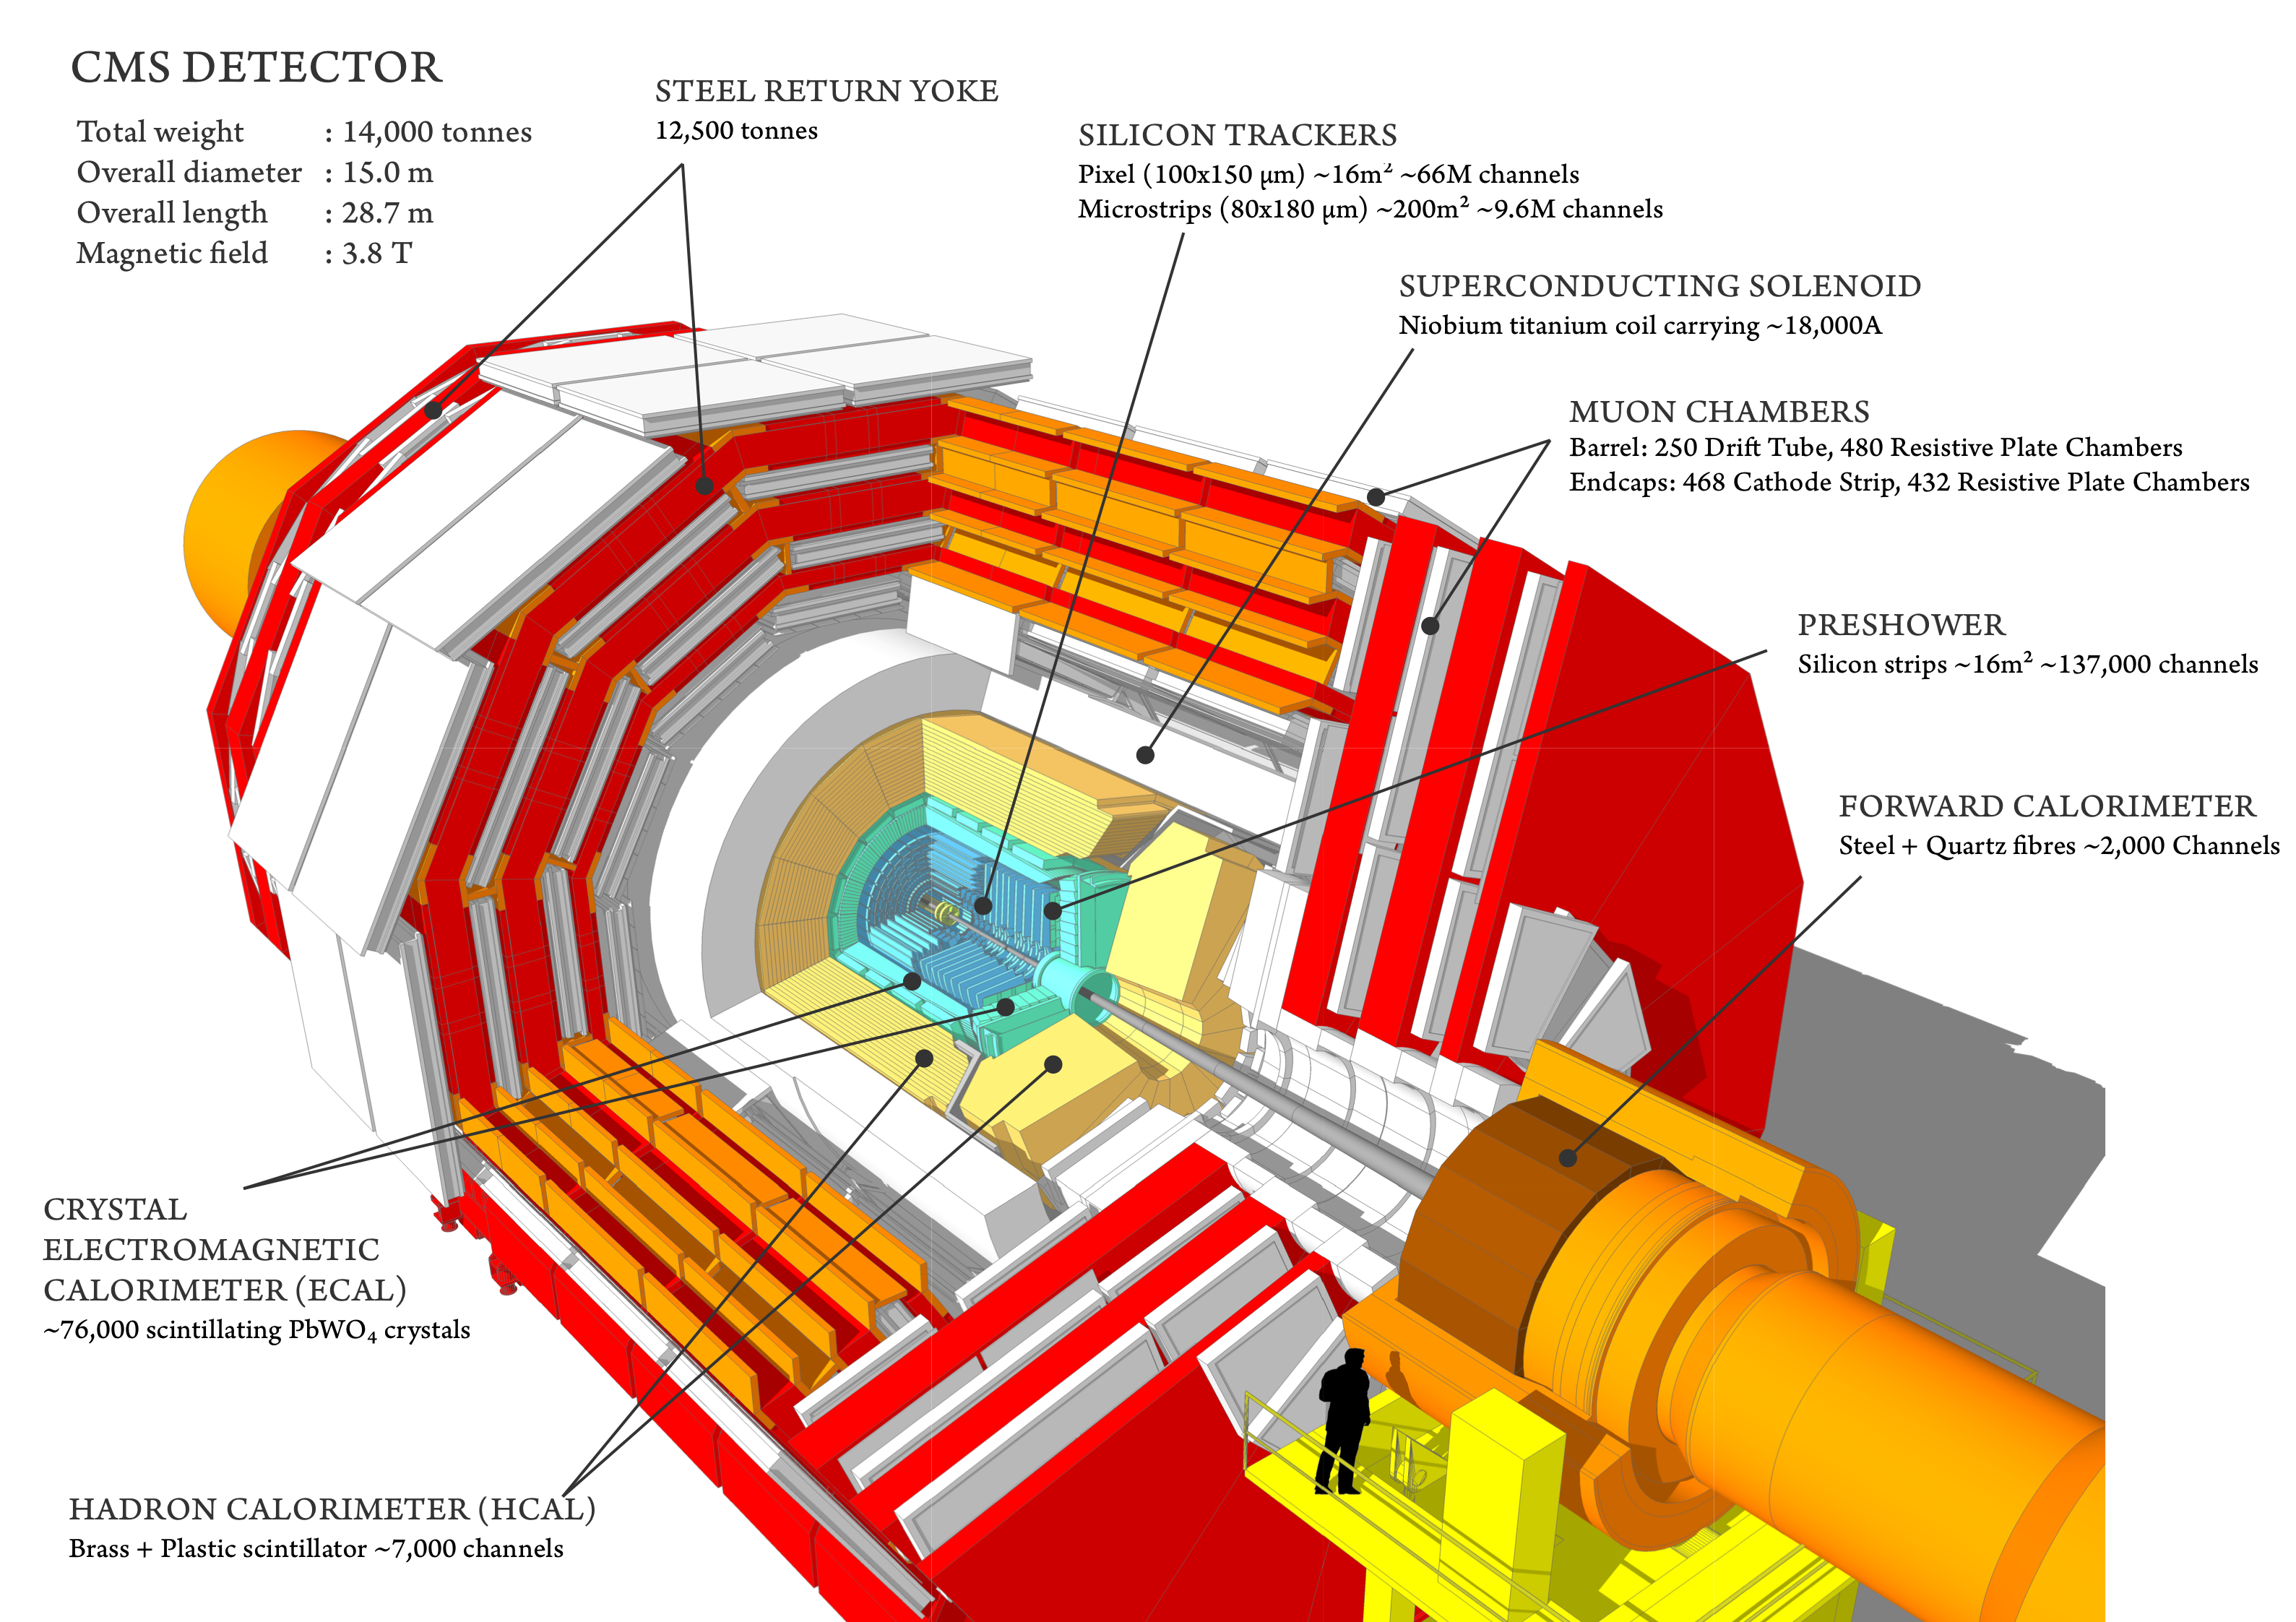
\includegraphics[width=0.8\textwidth]{plot/cms_layout.png}
	\caption{A perspective view of the CMS detector.}
	\label{fig:cmslayout}
\end{figure*}

The CMS uses a coordinate system with the origin centered at the interaction point. The positive y-axis is chosen to be the vertically upward direction, and the x-axis points toward the center of the LHC. Therefore the z-axis is pointing along the anti-clockwise beam direction. Cylindrical coordinates (r,$\phi$) are often used to describe the transverse plane, with $\phi$ being the azimuthal angle measured from the x-axis and r being the radial coordinate in the plane. The momentum and energy in the transverse plane, denoted as $p_T$ and $E_T$, are usually used as kinematic variables for physics objects, because the transverse components are invariant under Lorentz boosts in the z-direction. The polar angle $\theta$ is measured from the z-axis, and the pseudorapidity is defined as: 
\begin{equation}
	\centering
       \eta = -\text{ln tan}(\theta/2).
\end{equation}


\subsection{The Inner Tracking System}
The tracking system is designed to provide a precise and efficient reconstruction of the trajectories of charged particles. 
At the same time, accurate measurements of secondary vertices and impact parameters are necessary for the estimation of the positions of primary vertices as well as the identification of heavy flavors. 
At the designed luminosity of the LHC, about 1000 particles are expected to hit the tracker at each bunch crossing. 
To keep the occupancy at around 1\% in such challenging operation conditions, pixelated detectors and micro-strip detectors are used at the small radii and large radii regions respectively. 
The sensors are solely made of radiation tolerant silicons. With a sensitive area of about 200 $m^2$, the CMS tracker is so far the largest silicon tracker.  

The tracker has a cylindrical volume of 5.8 m in length and 2.5 m in diameter, embedded in the homogeneous magnetic field of 3.8 T. 
A schematic view of the CMS tracker is shown in Fig. \ref{fig:tracker}. 
In the barrel region, the pixel detector consists of three cylindrical layers at radii between 4.4 cm and 10.2 cm and the strip tracker consists of ten layers extending to 110cm in radius. 
Both subdetectors are complemented by disks on each side, extending to 290 cm in z and covering a pseudorapidity range up to $|\eta| <$ 2.5. 

\begin{figure*}[!htb]
	\centering
	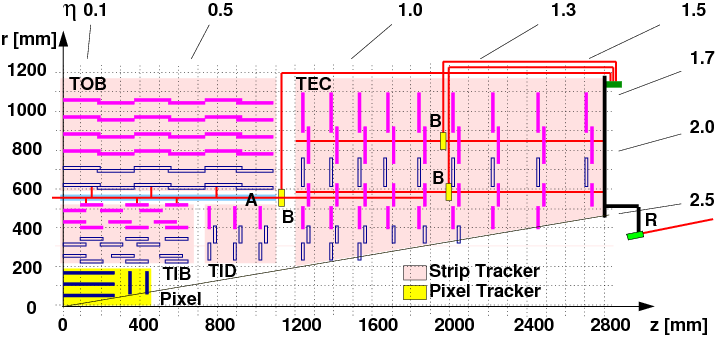
\includegraphics[width=0.8\textwidth]{plot/tracker.png}
	\caption{Layout of the CMS inner tracking system in an r-z view, showing the pixel detector and the silicon strip tracker.}
	\label{fig:tracker}
\end{figure*}


The pixel detector consists of three barrel layers located at radii of 4.4, 7.3 and 10.2 cm, closed by two disks on each side at z = $\pm$ 34.5 and $\pm$ 46.5 cm. 
It contains a total number of about 66 million silicon pixels with a cell size of 100 $\times$150 $\mu m^2$. 
It provides good track resolution in both the r-$\phi$ and z directions, allowing a three-dimensional (3-D) vertex reconstruction. 
It is essential for the identification of heavy flavors and forming seeds for the track finding.

Surrounded the pixel system is the strip tracker. 
It is composed of four subsystems. 
The Tracker Inner Barrel (TIB) and Disk (TID) extend to a radius of 55 cm, and are composed of four barrel layers and three endcap disks on each side. 
The sensors used by the TIB/TID are 320 $\mu m$ thick silicon micro-strips. 
The strips in the barrel are parallel to the beam pipe and have a pitch of 80 $\mu m$ on layer 1,2 and 120 $\mu m$ on layer 3,4, providing a position resolution of 23-35 $\mu m$. 
The disks use wedge-shaped sensors, with a pitch varies between 100 $\mu m$ and 141 $\mu m$. 
The innermost two layers of the TIB and the first two rings of the TID also carry a second module, mounted back-to-back with a stereo angle of 100 mrad, in order to measure the z (r) coordinate in the barrel (disks). 

The Tracker Outer Barrel (TOB) covers the radius from 55 cm to 116cm and consists of six barrel layers, with the innermost two layers having double-modules. 
The sensors are made of 500 $\mu m$ thick micro-strips, with pitches vary from 183 $\mu m$ to 122 $\mu m$. 
The TOB covers z $<$ 118 cm. The rest of the tracker volume is occupied by the Tracker Endcaps (TEC), composed of 9 disks on each side. 
300 $\mu m$ silicons are used on the inner fours rings, and 500 $\mu m$ thick strips are used in the outer rings. 

%Figure 5 shows the tracker material budget as a function of \eta, as estimated from simulation. The tracker modules, together with electronics, cooling and support structures, contribute a large amount of materials in the tracker volume and cause particles to interact before reaching the outermost layer of the tracker. 

Figure \ref{fig:pixelreso} shows the resolution of the pixel detectors during the Run-II operation.
A 8-10 $\mu m$ in $r-\phi$ and 20-25 $\mu m$ in z resolution is achieved in the pixel barrel and a 15-20 $\mu m$ resolution is achieved in the forward pixel detector.
Figure \ref{fig:stripreso} shows the resolution of the strip detectors. A 20-30 $\mu m$ in TIB and 20-45  $\mu m$ TOB hit resolution is achieved during Run-II operation.

\begin{figure*}[!htb]
	\centering
	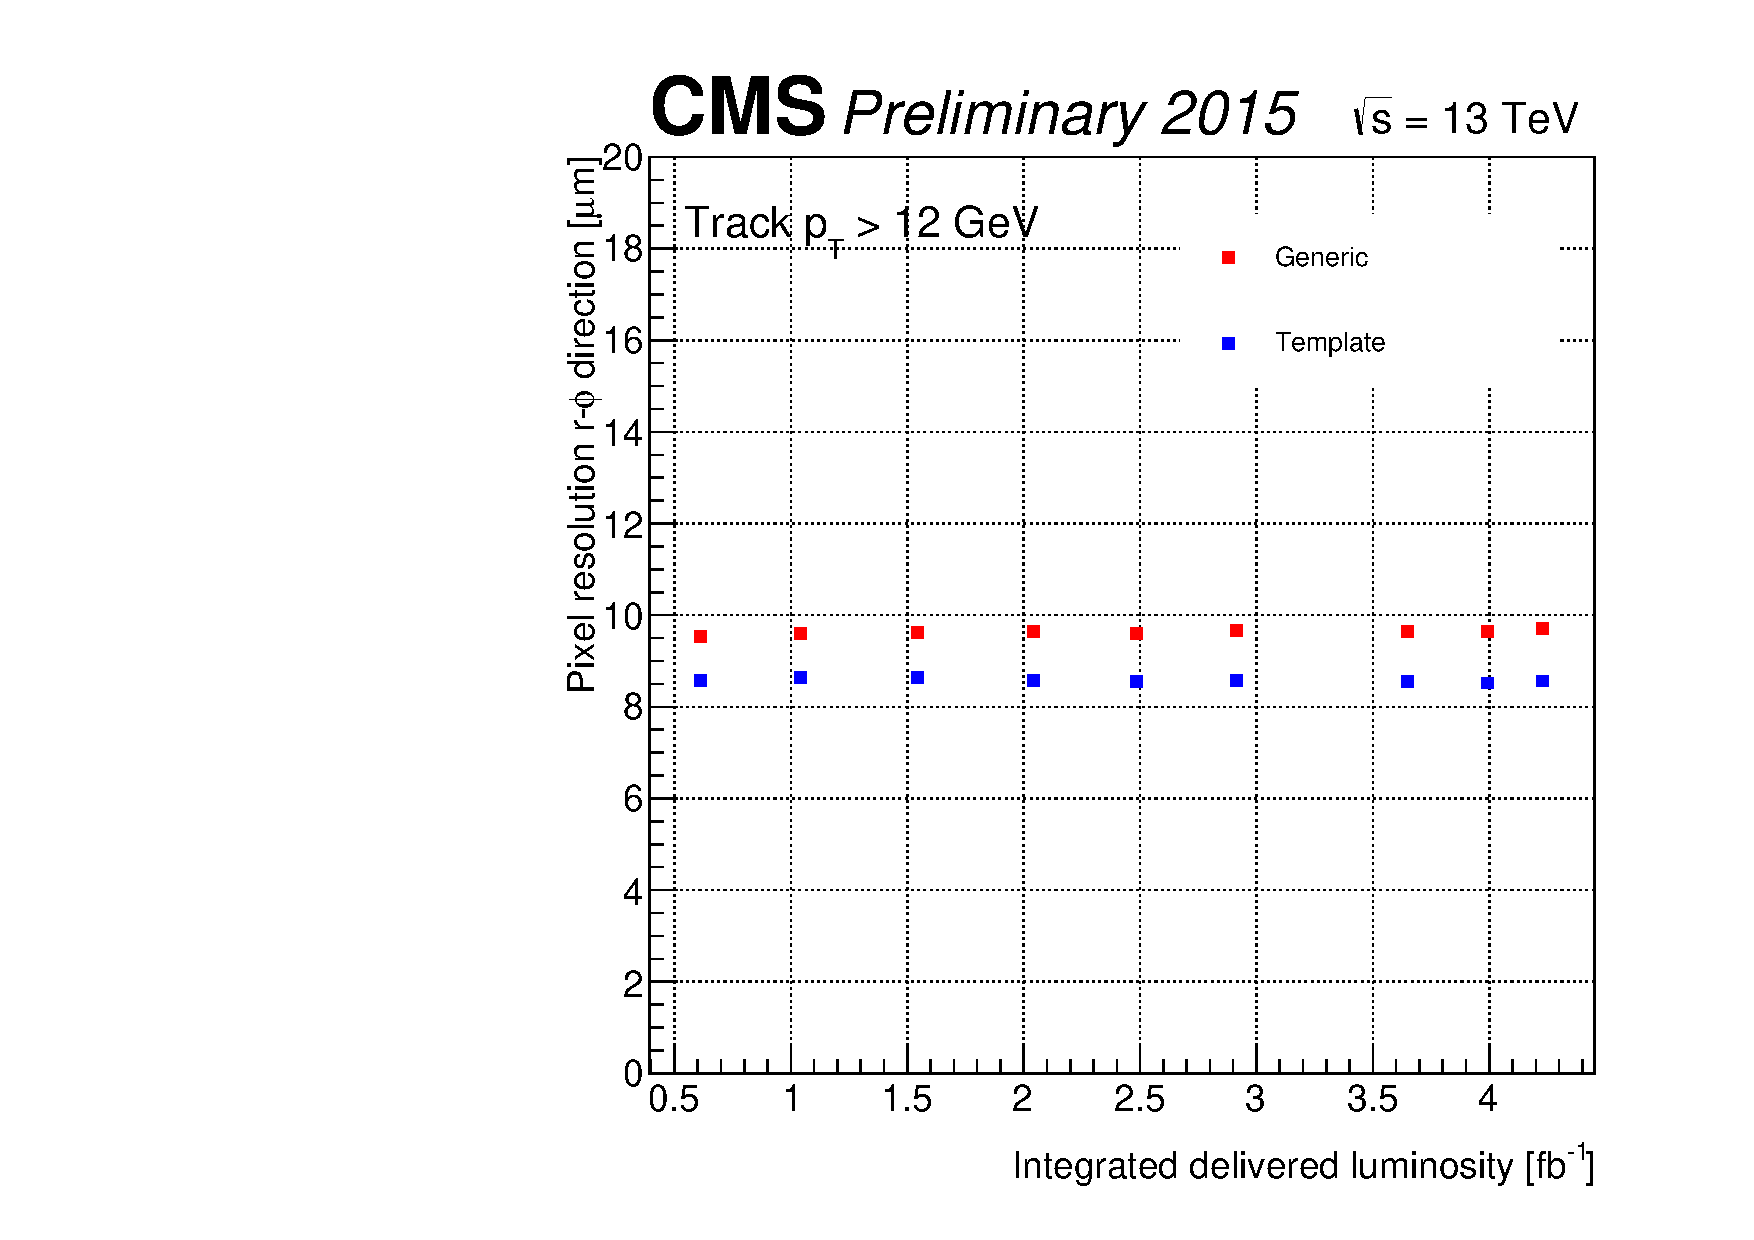
\includegraphics[width=0.49\textwidth]{Fig/LumiPlot_x_GenericVsTemplate_ReReco_3.pdf}
	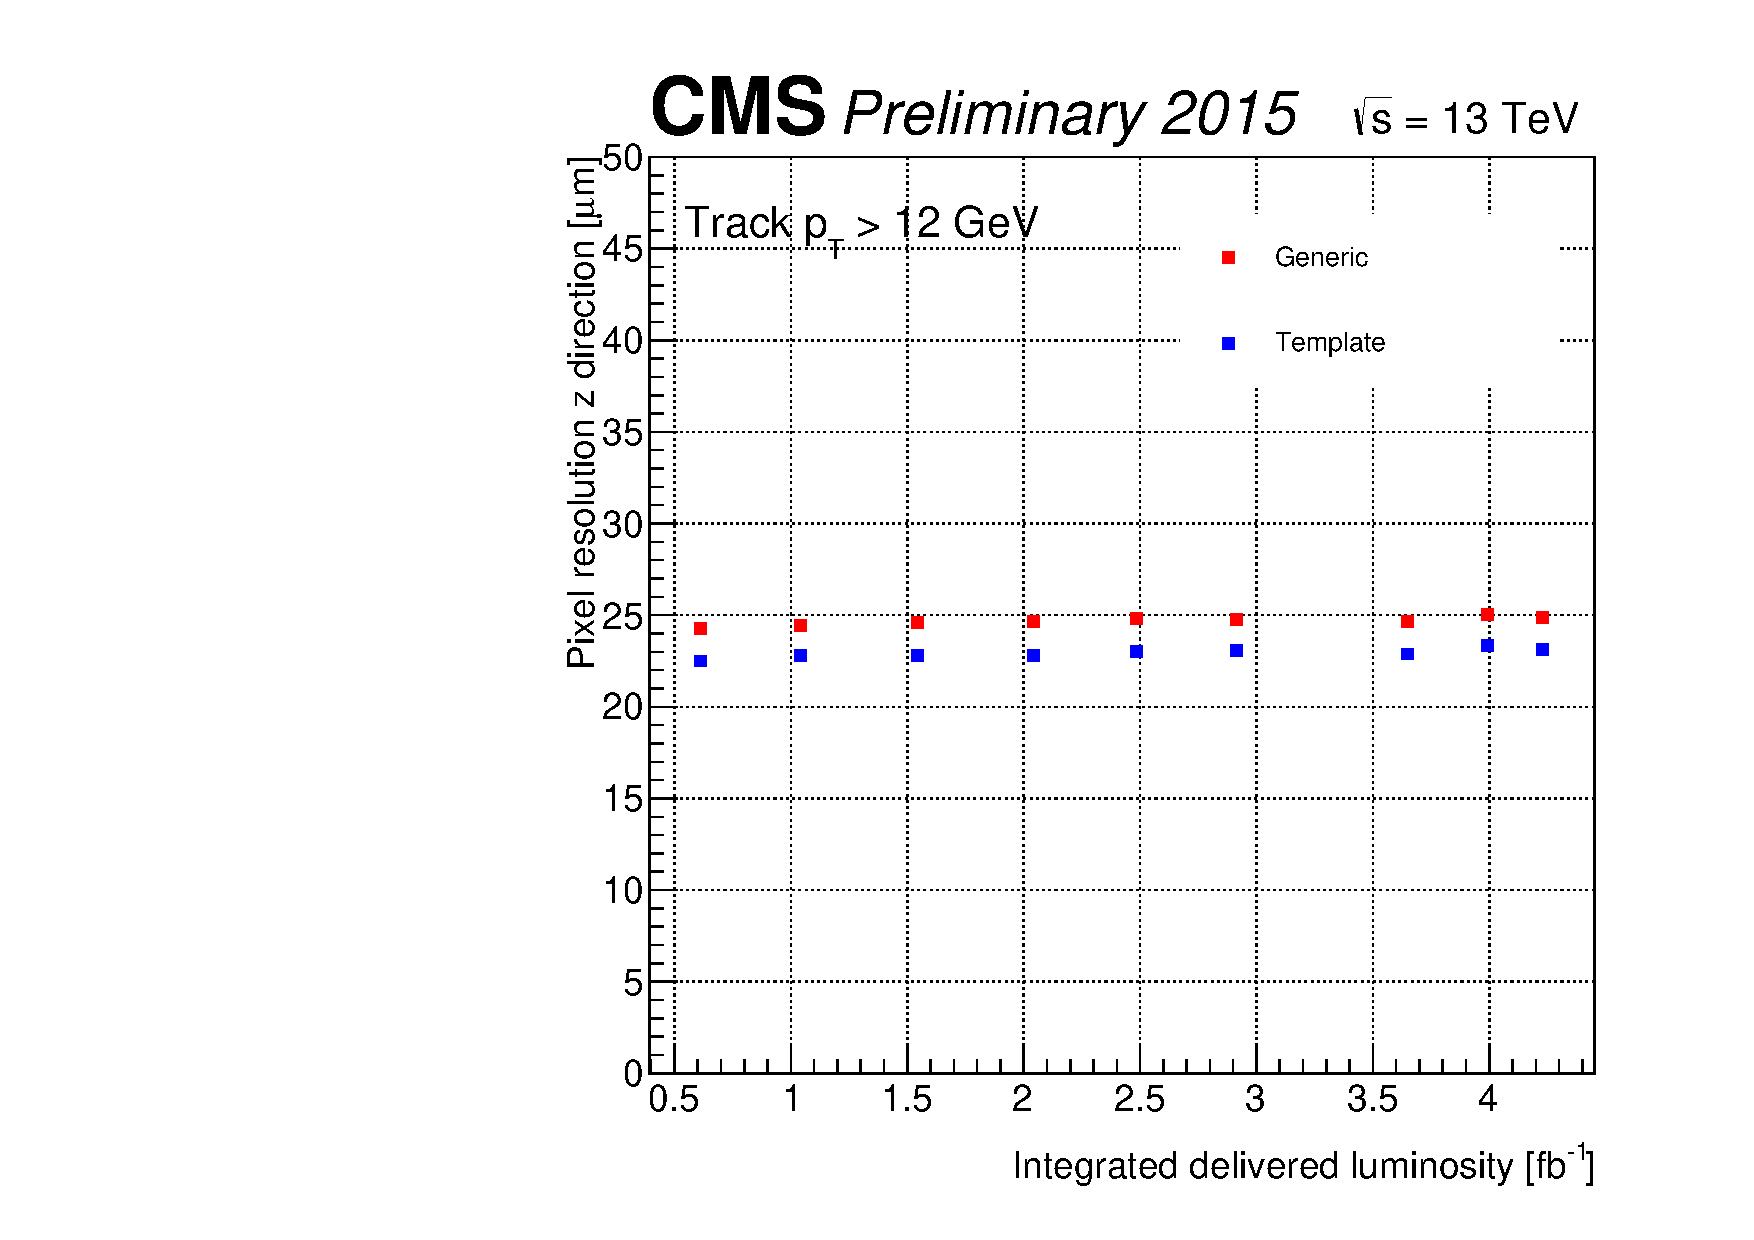
\includegraphics[width=0.49\textwidth]{Fig/LumiPlot_y_GenericVsTemplate_ReReco_3.pdf} \\
	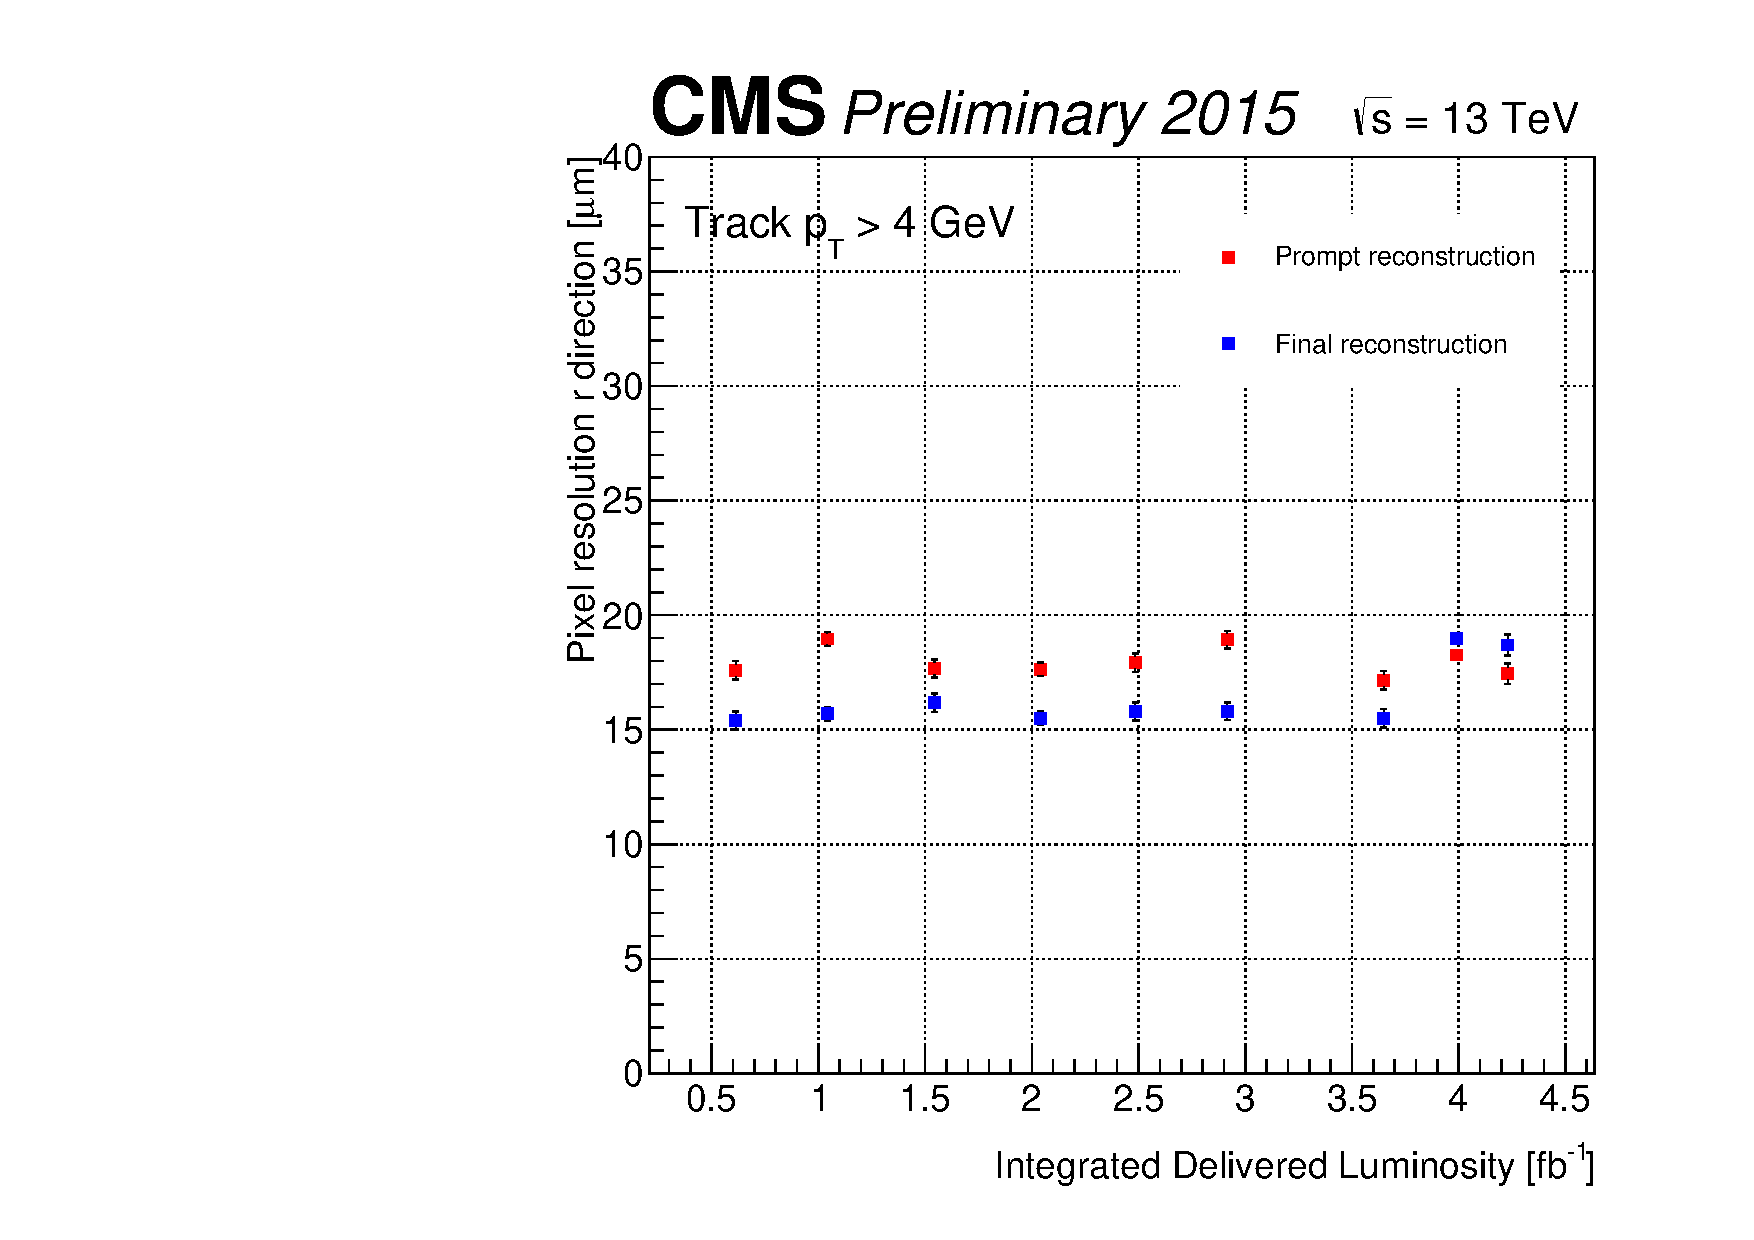
\includegraphics[width=0.49\textwidth]{Fig/LuminosityHistoryPlot_all_template.pdf}
	\caption{Evolution of the BPix resolution in r-$\phi$ direction (top left), BPix resolution in z (top right) direction, and the forward pixel resolution as a function of integrated luminosity in LHC Run II. Reprint from \cite{PixelPerformance}.}
	\label{fig:pixelreso}
\end{figure*}

\begin{figure*}[!htb]
	\centering
	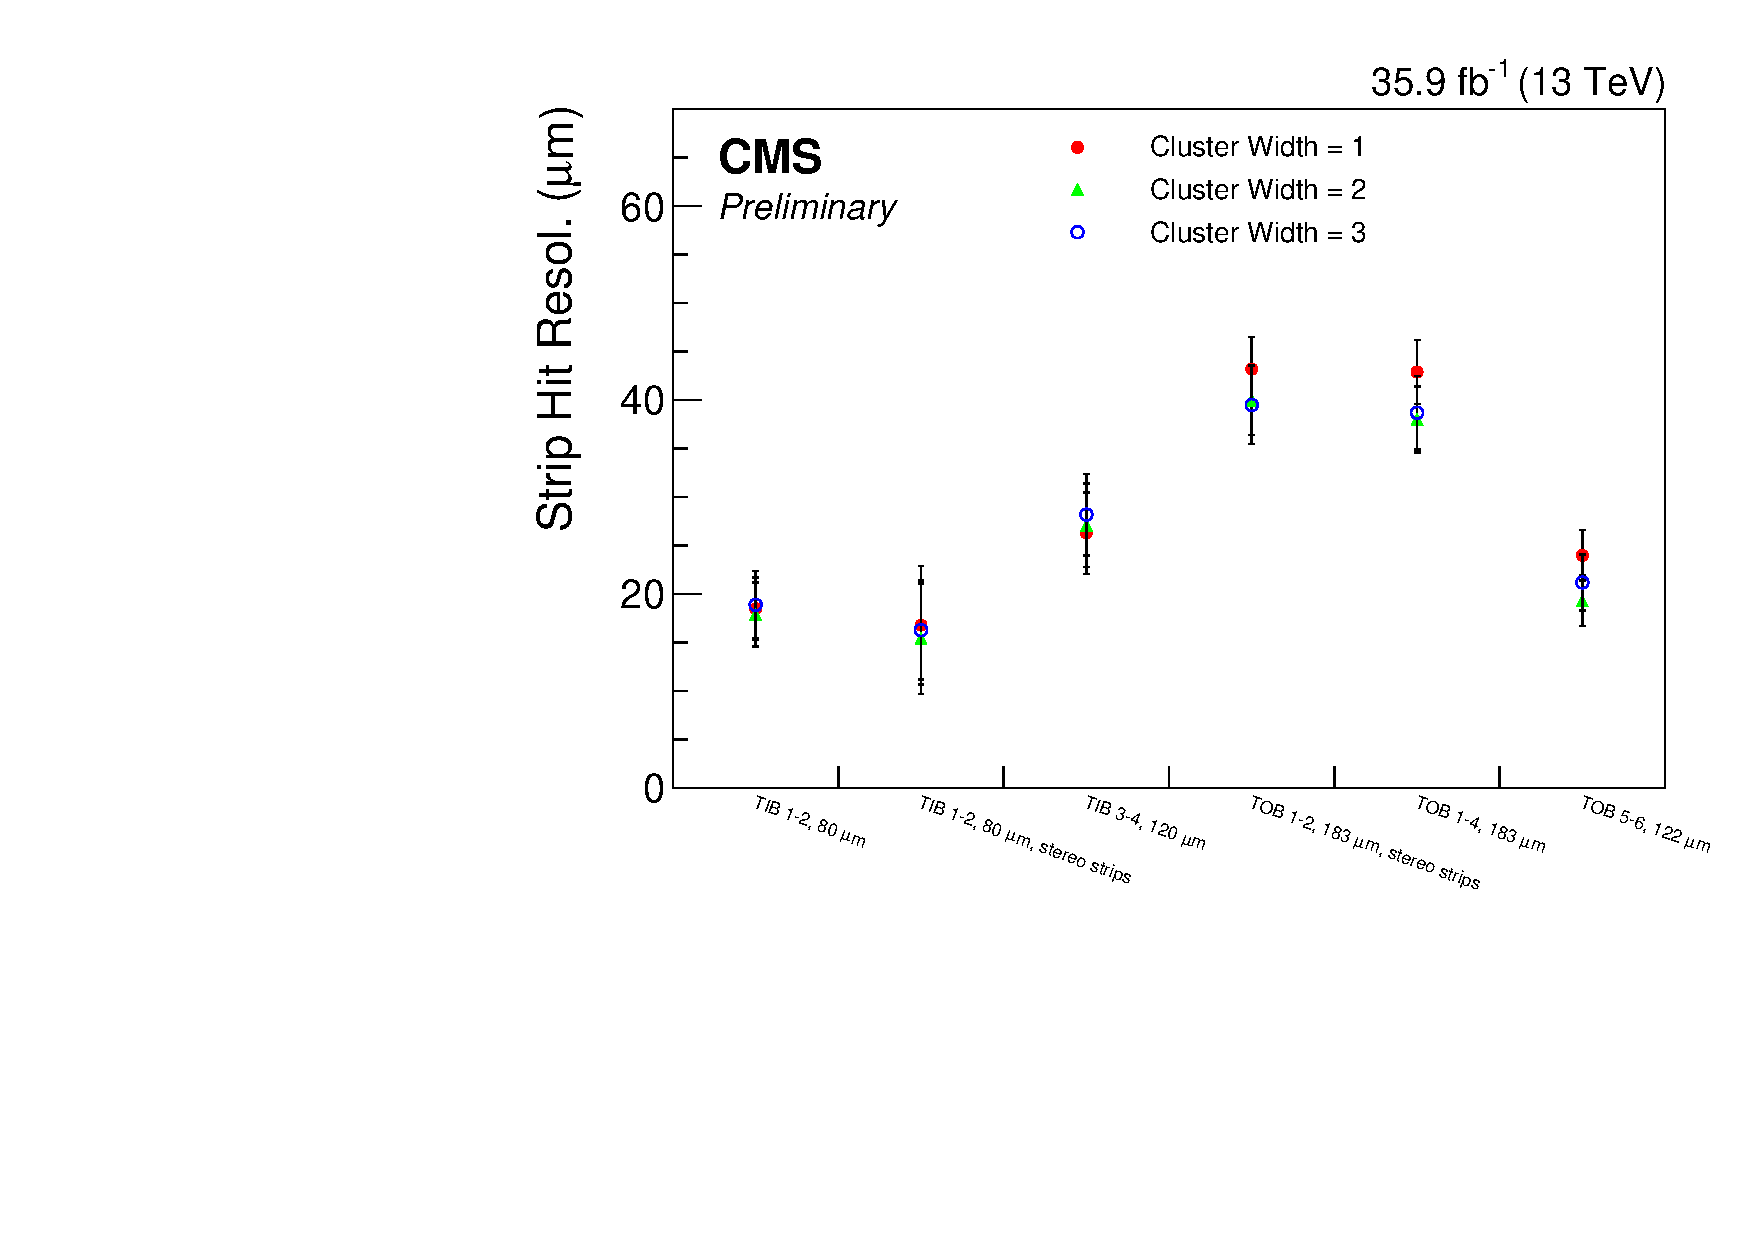
\includegraphics[width=0.49\textwidth]{Fig/StripHitRes.pdf}
	\caption{Strip Hit resolution for different cluster widths expressed in units of number of strips. }
	\label{fig:stripreso}
\end{figure*}

\subsection{Electromagnetic Calorimeter}
The CMS electromagnetic calorimeter (ECAL) is a hermetic, homogeneous detector consisting of 61,200 PbWO$_4$ crystals in the barrel (EB), and 7324 crystals in each of the two endcap sections (EE). 
The PbWO$_4$ crystals have a density of 8.28 g/cm$^3$, radiation length of 0.89 cm and Moli`ere radius of 2.2 cm. 
These characteristics make them the appropriate material for a compact calorimeter. 
The scintillation light emitted by the crystals are blue-green color, with a maximum wavelength at 420-430 nm. 
Therefore blue laser can be used to monitor the transparency and response of the crystals. 

The scintillation light is collected by avalanche photodiodes (APDs) in the barrel section and vacuum phototriods (VPT) in the endcaps. 
Each barrel crystal has one pair of APDs glued to its back face, and each endcap crystal has only one APT mounted. 
The photodetectors are depleted by a custom high voltage (HV) power supply which can precisely control the bias voltage and allow the gain of the photodetectors to be stable. 

A schematic drawing of the layout of the ECAL is shown in Figure \ref{fig:ecalall}. 
The EB uses 230 mm long crystals, corresponding to a radiation length of 25.8 $X_0$, while the length of the crystals in the EE is 220 mm (24.7 $X_0$). 
The crystals in the EB are grouped into 36 supermodules (SM), 18 on each side of the interaction point, and provide a granularity of 360-fold in $\phi$ and (2$\times$85)-fold in $\eta$, covering the pseudorapidity range up to $|\eta| <$ 1.479. 
The EE is composed of two Dees, each consists of 3662 crystals, and extends the coverage to $|\eta| = $3.0. 
In addition, a preshower (ES) detector made of lead absorbers and silicon strip sensors is placed in front of EE to improve the identification of closely spaced photons from $\pi^0$ decays. 

\begin{figure*}[hbt]
	\centering
	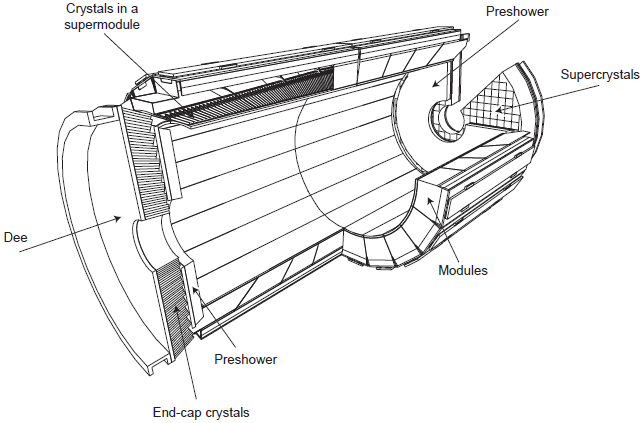
\includegraphics[width=0.8\textwidth]{Fig/The-CMS-Electromagnetic-Calorimeter-ECAL-The-barrel-section-comprises-36.png}
	\caption{Layout of the CMS Electromagnetic Calorimeter (ECAL).}
	\label{fig:ecalall}
\end{figure*}


The signals from the photodetectors are shaped and amplified by the Multi Gain Pre-Amplifier (MGPA) with gains of 1, 6 and 12. 
If the signal is saturated, the read-out will switch to a lower gain. 
Each of the output signals of the MGPA is digitized by a 12-bit analog-to-digital converter (ADC) running at 40MHz and a set of 10 consecutive samples is recorded for amplitude reconstruction.
The signals from a trigger tower ( $5\times5$ crystals ) in the EB or a super-crystal in the EE are read out together by the on-detector electronics and are stored in pipelines during the Level-1 trigger latency. 
Once a Level-1 trigger is received, the data will be sent out to the off-detector electronics. 

Radiation can cause a degradation in the crystal transparency due to the formation of color centers. 
The response of the VPT also varies under irradiation. 
In absence of irradiation, the transparency loss can partially recover through spontaneous annealing. 
These response changes are measured and corrected using a laser-based light monitoring system during the LHC operation. 
Blue and green laser light pulses are injected via optical fibers to the crystals and off-detector silicon PN photodiodes. 
The relative responses are then normalized to the measurements at the start of the run to derive correction coefficients. 
Figure \ref{fig:lasermonitor} shows the evolution of the ECAL response for the Run I and Run II 2016 data taking periods. 

\begin{figure*}[hbt]
	\centering
	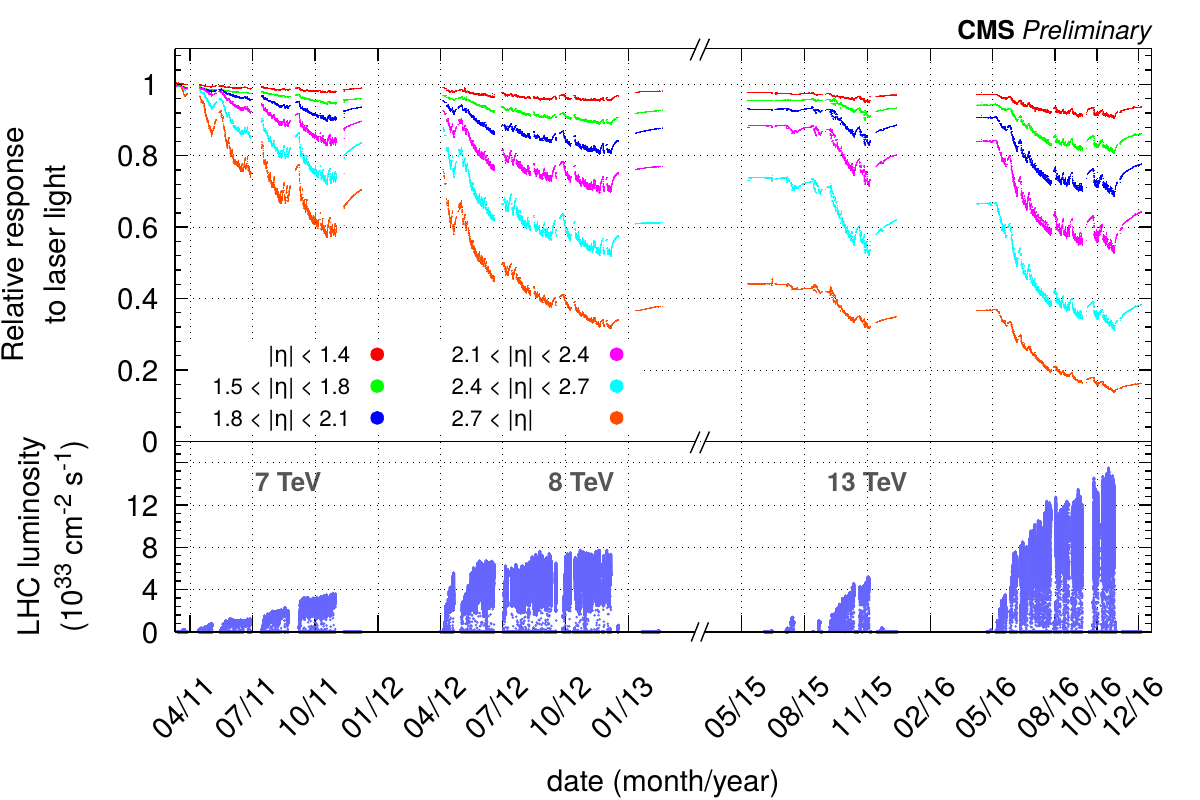
\includegraphics[width=0.8\textwidth]{Fig/lasermonitor.png}
	\caption{Evolution of the ECAL relative response as a function of data taking period.} 
	\label{fig:lasermonitor}
\end{figure*}

The ECAL has been operating stably throughout the 2015 and 2016 LHC Run II operation.
The analysis using 2.5fb collision data collected in 2015 shows that a relative energy resolution
between 1.4\% and 3\% for electrons is achieved in the EB, and 3\% to 4\% for EE~\cite{Sun:2233637}. 

\subsection{Hadron Calorimeter}
The hadron calorimeter (HCAL) is designed to absorb and measure the energy of hadrons. 
In addition, it is important for the indirect measurement of weakly interacting particles such as neutrinos which escape the detector and result in imbalanced momentum.
It contains four parts: a barrel (HB) with pseudorapidity range $|\eta| < $ 1.3, two endcaps (HE) covering 1.3 $ < |\eta| <$ 3.0, an outer calorimeter (HO) outside the solenoid to catch the shower tails, and two forward calorimeters (HF) positioned at either end of CMS.
Figure \ref{fig:hcal} shows the location of the HCAL in CMS detector. 

\begin{figure*}[hbt]
	\centering
	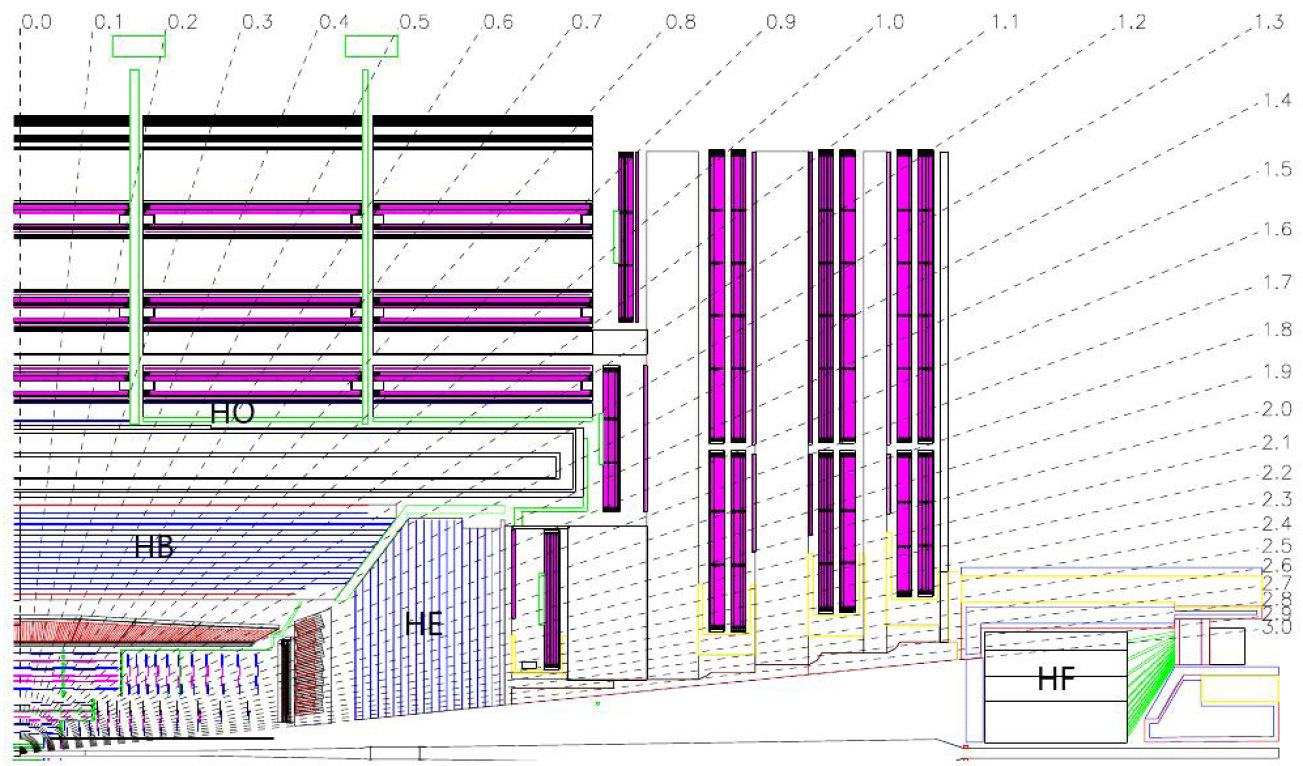
\includegraphics[width=0.8\textwidth]{plot/hcal.png}
	\caption{HCAL tower segmentation in the r-z plane.}
	\label{fig:hcal}
\end{figure*}

The HB and HE are the major sub-detector of the HCAL. 
They are sampling calorimeter made of alternating layers of brass absorber plates and plastic scintillator tiles.
The HB consists of 17 layers of absorber/scintillator, corresponding to a total interactions length of 5.39 at $|\eta| =$ 0 and 10.3 at $|\eta| =$ 1.3.
Each HE has 18 scintillator and 17 absorber layers, where the absorber is designed to minimize the cracks between HB and HE. 
When particles deposit energy in the HCAL, the active materials are excited by ionizing radiation and generate scintillation light, which is read out by wavelength shifting fibers. 

The optical signals are amplified and converted into electronic signals by multichannel Hybrid Photodiodes (HPDs). 
The output analogue signals are then digitized by the charge-integrator and encoder (QIE) chips. 
After digitization, the signals are delivered to the trigger/read-out (HTR) board of the backend electronics located in the service cavern. 
In the HTR, trigger primitives are generated and sent to the Regional Calorimeter trigger.
The HTR also buffers the readout data and transfers it to the data acquisition system when a Level 1 acceptance decision is received.  

Because of the geometric constraints of the solenoid coil, the EB plus HB doesn't provide enough materials to fully contain the hadron showers. 
To ensure adequate sampling depth in the $|\eta| < $ 1.3 region, the HO is placed outside the solenoid to detect any late showers or leakage from HB. 
The HO contains one layer of scintillator and utilizes the solenoid coil as absorber, extending the total interaction length of the calorimeter system to be at least 11.8 $\lambda_I$. 

In the forward region, the HF calorimeter extends the coverage up to $|\eta| < $ 5.2.
The design of the HF is very challenging due to the extremely high radiation dose near the beampipe.  
Therefore the HF is made up of radiation hard quartz fibers embedded within a 165-cm-long steel absorber.  
Signals are generated when charged particles above the threshold (0.2 MeV for electrons, 400 MeV for protons) emit Cherenkov lights in the quartz.
The lights are transported to photomultiplier tubes (PMT) for readout. 
The HF tower occupancy can be used for CMS luminosity measurements. 

\subsection{The Muon System}
The detection of muon is an important task of CMS, as suggested by the name of the experiment. 
Many interesting physics processes, including the decay of Higgs boson to $ZZ$ and potential production of new particles, may involve muons in the final states.
Muons are less affected by radiative losses because they are 200 times heavier than electrons.
Most of the muons can penetrate the calorimeter system with little interaction. 
Therefore the sub-system to detect the muons are placed in the outmost part of the CMS where other particles except neutrinos are expected to be fully absorbed.

The CMS muon system is designed to precisely measure the momentum and charge of muons over a wide kinematic range.
The detectors sit in between the segments of iron return yoke of the CMS solenoid, where the magnetic field is below 2 T, as shown in the Figure \ref{fig:magnet}.
Because of the large coverage area outside the solenoid, the materials of the muon system have to be cost-effective and robust.
Thus gas-ionization detectors are chosen to measure the muons. 
The muon system uses three different technologies: drift tubes (DT) in the barrel section, cathode strip chambers (CSC) in the endcaps, and resistive plate chambers (RPC) in both the barrel and endcaps to provide fast triggers.

\begin{figure*}[hbt]
	\centering
	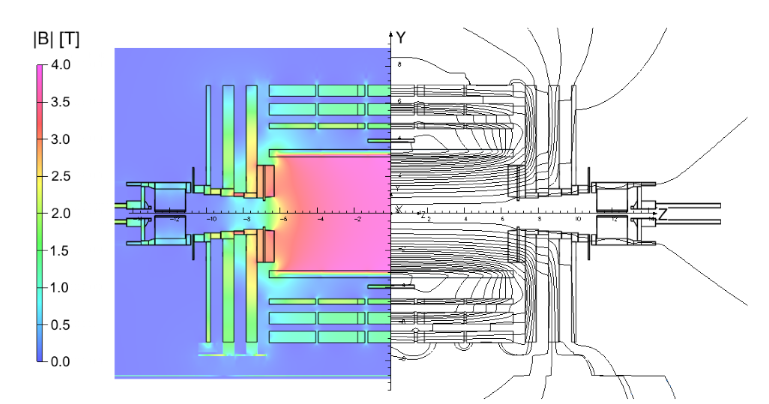
\includegraphics[width=0.8\textwidth]{plot/magnet.png}
	\caption{Map of the magnet field (left) and field lines (right) predicted for a longitudinal section of the CMS detector by a magnetic field model at a central magnetic flux density of 3.8 T. Each field line represents a magnetic flux increment of 6 Wb}
	\label{fig:magnet}
\end{figure*}

\noindent \textbf{Drift Tubes} 

The muon rate and radiation dose in the central region are relatively low, thus the drift tubes are used in the barrel to cover the pseudorapidity region up to $|\eta| < $ 1.2.
The DT is a closed-cell wire chamber which consists of a thin wire at high positive voltage (anode) within a gas-filled volume.
When charged particles pass through the chamber, gas atoms will be ionized and the resulting electrons will drift towards the anode wire.
The hit position of the muons can be reconstructed by measuring the drift time.  

The basic element of the DT is a rectangular drift cell with a transverse cross-section of $42 \times 13\ mm^2$. 
A gold-plated stainless-steel wire is suspended in the center of the chamber and operates at +3600 V. 
Four parallel layers of such drift tubes are staggered by half a cell to form a superlayer (SL). 
SLs with wires along the beam direction can provide measurements for $r\text{-}\phi$ coordinates, while orthogonal SLs can measure the $r\text{-}z$ coordinates. 
The barrel muon detector consists of four concentric DT stations interleaved with iron yokes, as shown in Figure \ref{fig:DT}.
Each of the inner three stations, labeled as MB1, MB2, MB3, has 60 chambers which consist of two parallel SLs and one perpendicular SL. 
The outer station has 70 chambers, however, each chamber has only an $r\text{-}\phi$ SL. 

The single-hit spatial resolution of the DT tube is averagely 260 $\mu m$ in the $r\text{-}\phi$ direction.
When segments of the whole chamber are fitted together, the resolution is improved to be 90 $\mu m$.

\begin{figure*}[hbt]
	\centering
	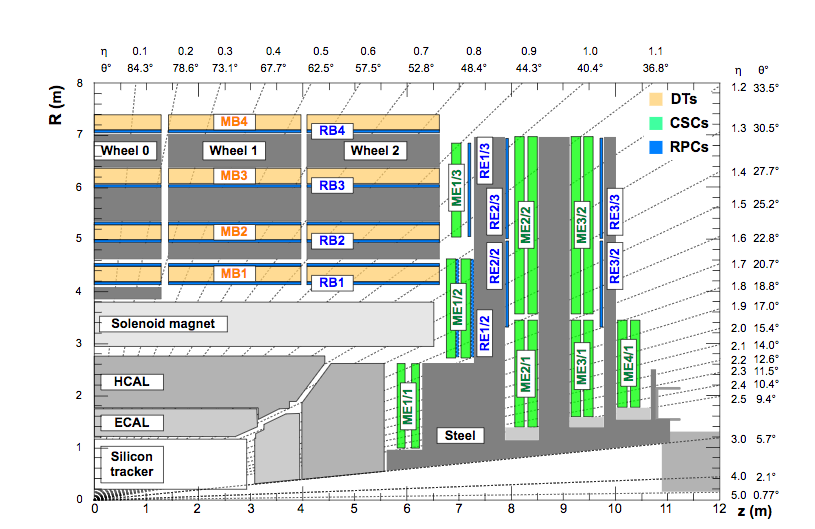
\includegraphics[width=0.8\textwidth]{plot/DT.png}
	\caption{An R-z cross section of a quadrant of the CMS detector with the axis parallel to the beam (z) running horizontally and radius (R) increasing upward.  The interaction point is at the lower left corner. 
	 Shown are the locations of the various muon stations and the steel disks (dark grey areas). The 4 drift tube (DT, in light orange) stations are labeled MB (?muon barrel?) and the cathode strip chambers (CSC, in green) are labeled ME (?muon endcap?).              Resistive plate chambers (RPC, in blue) are in both the barrel and the endcaps of CMS, where they are labeled RB and RE, respectively.}
	\label{fig:DT}
\end{figure*}

\noindent \textbf{Cathode Strip Chambers}

In the endcap region, the muon rate is higher and the magnetic field is non-uniform.
Thus the cathode strip chambers are chosen to measure the muons in the endcaps since they have a faster response time. 
The CSC is another type of multiwire chamber which consists of thin parallel anode wires crossed with negatively-charged cathode strips.
All chambers are filled with a gas mixture of 50\% CO$_2$, 40\% Ar, and 10\% CF$_4$.
When charged particles pass through, they ionize the gas and produce free electrons, which move to the anode wires creating an avalanche pulse.
Positive ions move to the cathode strips and induce a pulse so that a pair of position coordinates can be read out from one individual chamber.
Six such chambers form a CSC module, allowing a precise measurement of muon tracks. 

Each endcap has 4 CSC stations, containing a total of 468 chambers.
The chambers are mounted on the surface of endcap disks in a way that the cathode strips run radially and the anode wires measure the $r$ coordinate. 
The full CSCs provide a coverage of the pseudorapidity from 0.9 to 2.4.
A reconstruction efficiency of 96-99\% is achieved for muons except in the gap regions.

\noindent \textbf{Resistive Plate Chambers}

The gaseous detectors with wires can provide excellent spatial resolution, however, the time resolution is relatively poor because of the fluctuations in drift time. 
The time resolution can be improved using detectors with intense electric field so that the amplification of the signals can immediately start after primary ionization. 
To ensure unambiguous identification of the collision bunch at the highest LHC luminosities, a dedicated trigger detector made of resistive plate chambers (RPC) is implemented to complement the DTs and CSCs.

The RPCs are double-gap parallel-plate detectors, each gap consists of two plates made of high resistive plastic material. 
The outer surfaces of the plates are coated with conductive graphite paint, and a voltage of 9.6 kV is applied, allowing the RPCs to operate at avalanche mode.
The use of high resistive electrode limits the discharge of the chamber to a small region so that the deadtime of the full detector is negligible and a good efficiency is ensured.

The RPCs are installed in both the barrel and endcap region, covering a pseudorapidity region $|\eta| <$ 2.1.
There are four RPC stations in the barrel, of which the innermost two stations consist of 2 layers of RPCs with DT sandwiched. 
In the endcap region, there were 3 RPC stations in LHC Run I. 
During the first long shutdown (LS1), an additional 144 RPCs are installed to the fourth disk. This improved the muon reconstruction efficiency in the range 1.2 $< |\eta| < $ 1.8. 

The RPC system operated smoothly during the LHC Run II with an average efficiency of 94\%. 
A time resolution of 3 ns or better is achieved for all 3 systems~\cite{MuonPerform7TeV,MuonPerform13TeV}.


\section{CMS Trigger System}
The LHC provides proton-proton collisions every 25 ns, leading to an event rate of 40 MHz. 
The raw data per event is about 1 MB, which means 40 TB data is produced every second.  
This large amount of data is far beyond the ability of the machine to store and process the events. 
Moreover, the production rate of the interesting physics processes are a few orders of magnitude lower than the total pp collisions rates. 
Therefore, a data filtering system is needed to drastically reduce the event rate while keeping the interesting events recorded. 
This task is performed by the CMS trigger system.
The CMS trigger system reduces the event rate in two steps: the Level-1 trigger (L1) uses hardware electronics to reduce the data rate to 100 kHz, and the high level trigger (HLT) uses software to future reduce the rate to $\sim$ 1 kHz.\\

\noindent \textbf{Level-1 Trigger}

The L1 trigger receives coarsely segmented data from the sub-detectors and performs rough reconstruction of the particles using programmable electronics (FPGA, ASICs).
It consists of local and global components. 
The scheme of the L1 system is shown in Figure \ref{fig:L1}.
In the local trigger level, energy deposits in the calorimeters and hits in the muon stations are summed with reduced resolution to generate trigger primitives (TP). 
The TPs are fed into two trigger processing layers for object identification and global energy summation, and the resulting objects are sent to the global trigger (GT) for the final L1 decision.

\begin{figure*}[hbt]
	\centering
	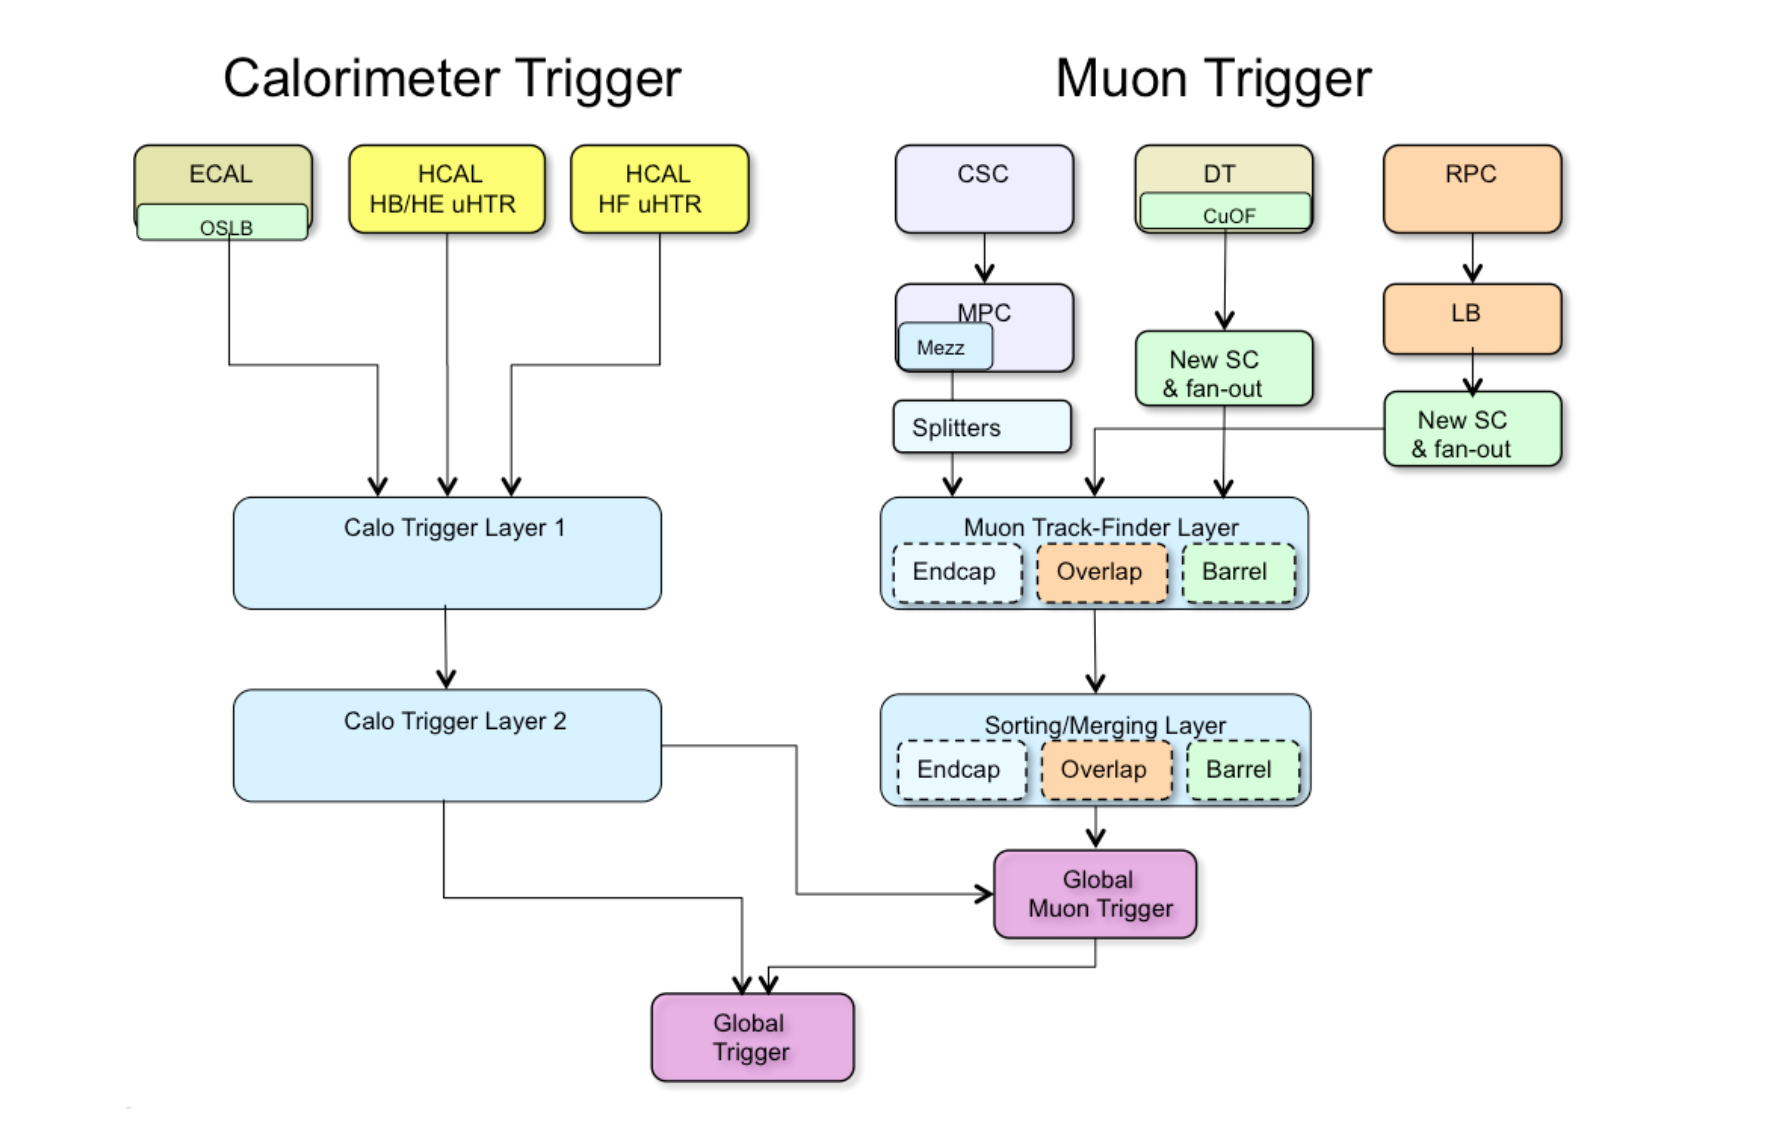
\includegraphics[width=0.8\textwidth]{plot/L1flow.png}
	\caption{Dataflow for the L1 trigger. Reprint from \cite{Tapper:1556311}.}
	\label{fig:L1}
\end{figure*}


The calorimeter trigger was upgraded during LHC LS1 to adopt a time-multiplexed system that enables the data from the entire calorimeter to be processed in a single FPGA at full granularity~\cite{Zabi}.
It consists of two layers, of which the first layer is designed to pre-process the TPs from ECAL and HCAL and format the data for layer 2.
The second layer is the main processing layer that performs the object identification and energy reconstruction. 
$e/\gamma$ candidates are reconstructed by dynamic clustering algorithms around local energy maxima above a fixed threshold. 
Trigger level energy calibration factors are applied to both the TPs and $e/\gamma$ objects in order to make the summed energy to be similar to the offline reconstructed energy. 
Jet candidates are formed by taking 9 $\times$ 9 TTs sliding windows around the seed towers. 
Other global quantities, such as the transverse missing momentum, are computed using the full granularity.

The muon trigger system was also upgraded during LS1 to meet the increased luminosity of LHC Run II. 
Trigger level muon tracks are reconstructed in the track finder (TF) layer which is composed of three separate components: barrel muon track finder for the DT and RPC in $|\eta| < $ 0.83, the endcap muon track finder for RPC and CSC in $|\eta| > $ 1.24, and the overlap muon track finder covering the three subdetectors in region 0.83 $< |\eta| <$ 1.24. 
Candidates from the TFs will be propagated to the global muon trigger (GMT) for sorting and isolation computing. 
The selected muons will be sent to the global trigger (GT) along with the information from the calorimeter trigger.

GT is the last stage of the L1 trigger. 
L1 decision is made using information received from the calorimeter and muon triggers. 
The GT has been upgraded with state-of-the-art FPGAs on Advanced Mezzanine Cards in a MicroTCA crate.
The upgraded processors can compute different objects and higher level physics quantities, such as invariant mass, with high efficiency.
\\

\noindent \textbf{High Level Trigger}

The HLT is a software trigger running on a computing farm which consists of more than 10,000 CPU cores. 
The basic unit of the HLT menu is called a trigger path, which consists of a series of reconstruction sequences and event filters. 
Event selections of each trigger path start from requiring the presence of one or more L1 objects, which are called L1 seeds. 
When the L1 seeds pass the kinematic selections of the trigger path, object reconstruction will be performed sequentially with increased complexity so that simple and fast algorithms can run first in the trigger path. 
A list of filters are implemented in the trigger path to decide if an object/event should be tentatively accepted or rejected. 
There are more than 400 trigger paths implemented in HLT menu in Run II to cover a wide range of physics signatures.
An event is only recorded if it is accepted by at least one trigger path. 

The HLT paths are grouped into several output datasets called primary data sets. 
These data sets include data streams for both physics analysis and detector operations. 
The RAW data of each event is about 1 MB, while the storage manager can temporarily store the data on disk with a 2GB/s rate. 
Therefore the HLT rate is limited to 1000 Hz.
In Run II, the HLT reconstruction sequences are implemented with the Particle Flow algorithms, which improves the energy resolution and pile-up mitigation in the increased luminosity conditions. 

\section{The Data Quality Monitoring and Certification System}
The Data Quality Monitoring (DQM) system~\cite{DQMFEDE} is a histogram-based software toolkit that evaluates and records the data quality of each sub-detector.
The primary goal of the DQM system is to identify problems of each sub-detector and guarantee the quality of physics data. 
The DQM has an online instance as well as an offline instance. 
The online DQM receives a subset of the CMS data and performs a real-time analysis on these data in order to give immediate feedback about the detector and trigger status. 
The offline DQM, on the other hand, takes the full dataset as input and performs a more precise reconstruction and evaluation of the data than in the online instance.
The offline DQM is used in the monitoring of the reconstruction quality, validation of simulated data, and test new CMS software releases.

Figure \ref{fig:dqmworkflow} shows the workflow of the DQM. 
The subset of raw data containing both the physics events and calibration data are delivered to the DQM farm for unpacking and reconstruction.
Each sub-detector has a set of DQM code that check the quality of the data relevant to it and record the analysis results in a ROOT file.
The quality check is performed every lumi section, and the ROOT files are delivered to the graphical user interface (GUI) for view.
GUI, the central component of the DQM, is a website for browsing data quality histograms.
The content in GUI is organized in workspaces depending on the scope and ranging from high-level summaries to shift views to expert areas.  

\begin{figure*}[hbt]
	\centering
	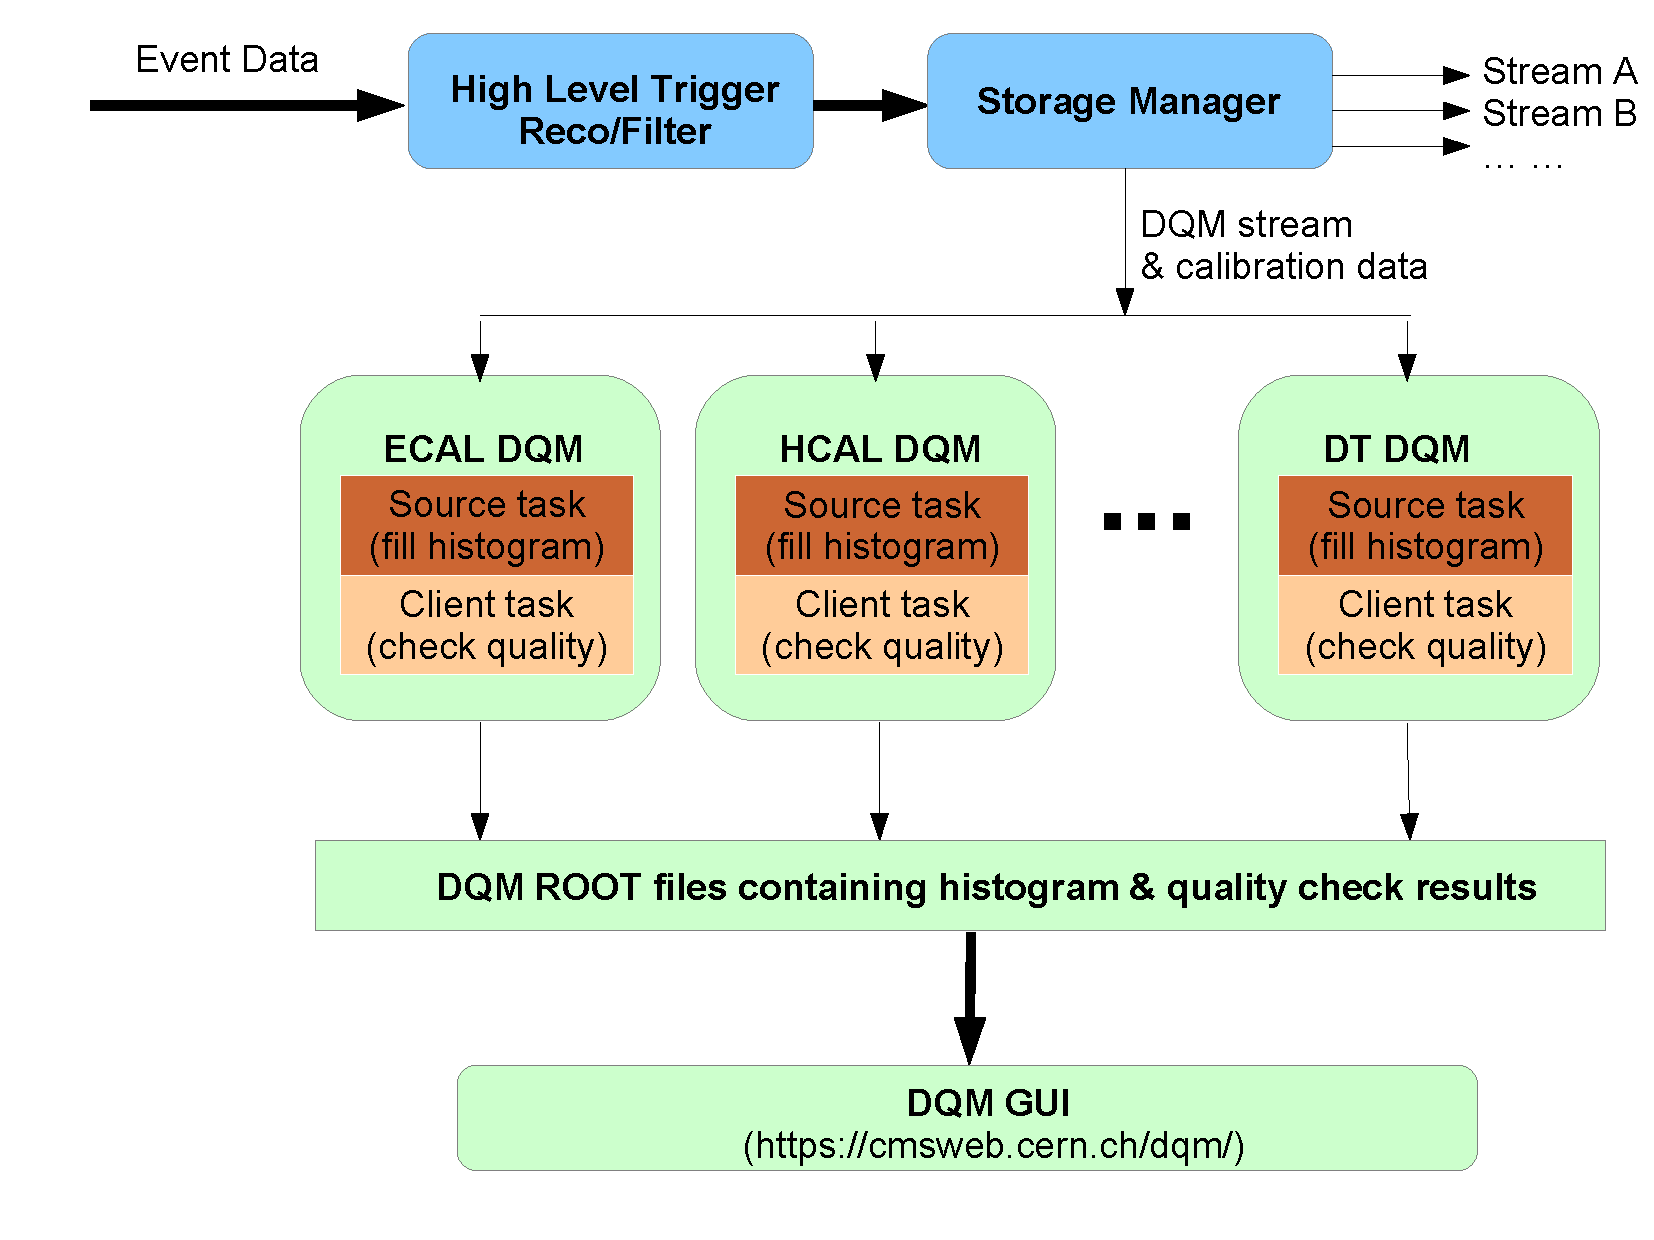
\includegraphics[width=0.8\textwidth]{Fig/DQMFlow.pdf}
	\caption{Workflow of the data quality monitoring system.}
	\label{fig:dqmworkflow}
\end{figure*}

A snapshot of the ECAL DQM GUI is shown in Figure \ref{fig:ecaldqm}.
It has access to both low level detector information, such as channel pedestals and noise, and high level data quality, like reconstructed hit timing. 
The values of pedestals and noise of the ECAL channels can be extracted from the DQM histogram and recorded into the CMS database, which are used for overall detector goodness check.
Besides the detector quality check, the DQM is also useful in a variety of analysis. 
For instance, the timing histograms in the ECAL DQM can be used to align the timing of different ECAL components. 

\begin{figure*}[hbt]
	\centering
	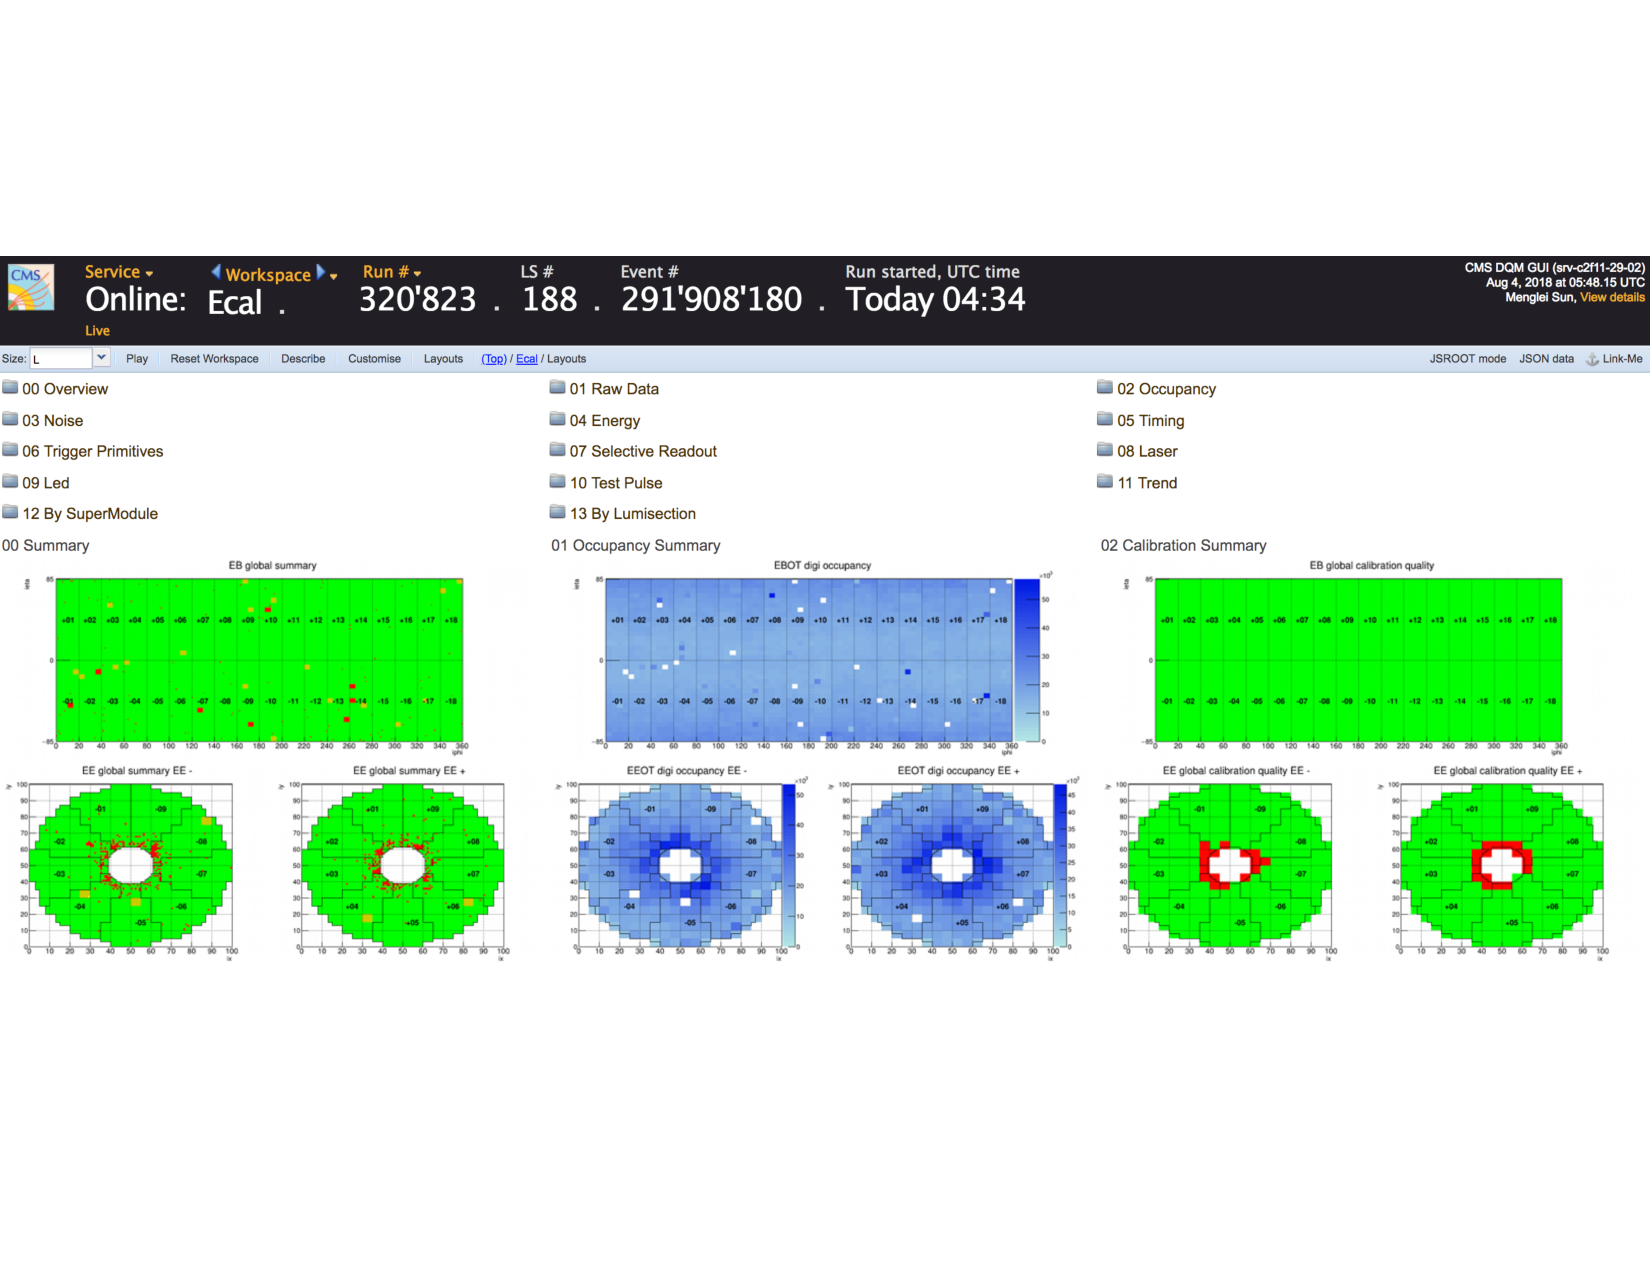
\includegraphics[width=0.8\textwidth]{Fig/ecaldqm.pdf}
	\label{fig:ecaldqm}
	\caption{Snapshot of the ECAL DQM.}
\end{figure*}

The DQM is in addition used in the certification of data good for physics analysis.
This process starts with the physicists checking the data quality of each lumi section using the offline DQM.
For each sub-detector a single boolean flag is used to describe the final quality result.
Once the quality check is done, the physicists will fill the basic run information along with the quality results in the run registry system, which is a dataset that bookkeeps the certification result.
If the data of all sub-detectors in a lumi section have good quality, this lumi section is certified to be good and its information is recorded in a JSON file which is used to select data for analysis. 

\end{document}


